%!TEX root = ../dissertation.tex
%\begin{savequote}[75mm]
%Nulla facilisi. In vel sem. Morbi id urna in diam dignissim feugiat. Proin molestie tortor eu velit. Aliquam erat volutpat. Nullam ultrices, diam tempus vulputate egestas, eros pede varius leo.
%\qauthor{Quoteauthor Lastname}
%\end{savequote}

\chapter{Evaluation and Results}
This chapter will explain the configuration of experiments for a Baseline model (Section \ref{sec:4-baseline}), Trivial Transfer Learning model (Section \ref{sec:4-trivial}), and Hierarchical Transfer Learning model (Section \ref{sec:4-hierarchical}). The findings of these experiments will be outlined within the pertaining section.
\newpage

\section{Experiments}

The Scottish Gaelic dataset consists of 145,000 sentences from the the original and back-translated data, as described in Table \ref{tab:low_resource-data}. The French dataset consists of 170,000 sentences from the data described in Table \ref{tab:available-data}. Finally the Irish Gaelic dataset consists of 170,000 sentences from the back-translated monolingual English data extracted from the Italian and Spanish data described in Table \ref{tab:available-data}.
All of the sentences fit within the maximum sentence length of 20 words and as mentioned in the methodology, during data pre-processing the source and target language vocabulary size have been limited to 7000 unique words, with prioritisation given to the most frequently occurring words. For the parent and intermediary languages, the test split been set to 0 and the validation split has been set to 0.1. This means that a significantly higher percentage of the available sentences are used for training.

\subsection{Vocabulary Size}
\label{sec:4-vocab_size}

To determine the most suitable vocabulary size for the Scottish Gaelic dataset, tests at sizes 4000, 5000, and 7000 were conducted. The maximum value was 7000 as the total vocabulary size with a minimum word occurrence of 2 was approximately 7000.
The vocabulary size of subsequent experiments will be determined by selecting the vocabulary size that returns highest \acrshort{BLEU} score. The validation loss of each size during training is shown in Figure \ref{fig:loss_vocab}.

\begin{figure}[ht!]
\centering
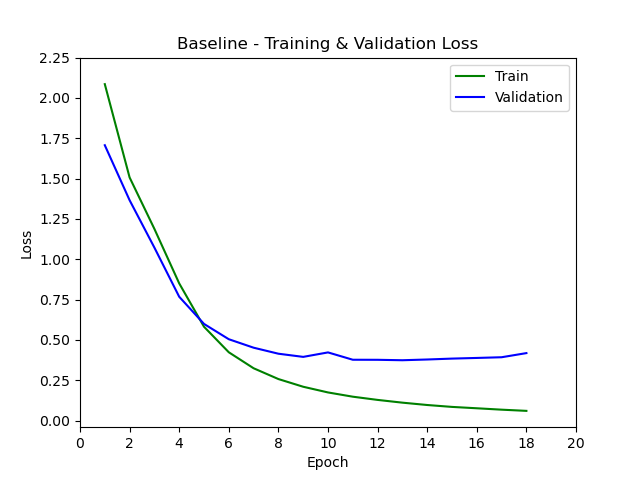
\includegraphics[width=0.6\textwidth]{media/experiments/loss/loss_baseline.png}
\captionsetup{justification=centering}
\caption[Baseline Model Vocabulary Size Validation Loss]{Baseline Model Vocabulary Size Validation Loss}
\label{fig:loss_vocab}
\end{figure}


\subsection{Baseline}
\label{sec:4-baseline}

The baseline translation model described in Section \ref{sec:3-model} has been trained for 20 epochs with a vocabulary size of 7000 using only the final Scottish Gaelic dataset. The training and validation loss can be seen in Figure \ref{fig:loss_baseline}.

\begin{figure}[ht!]
\centering
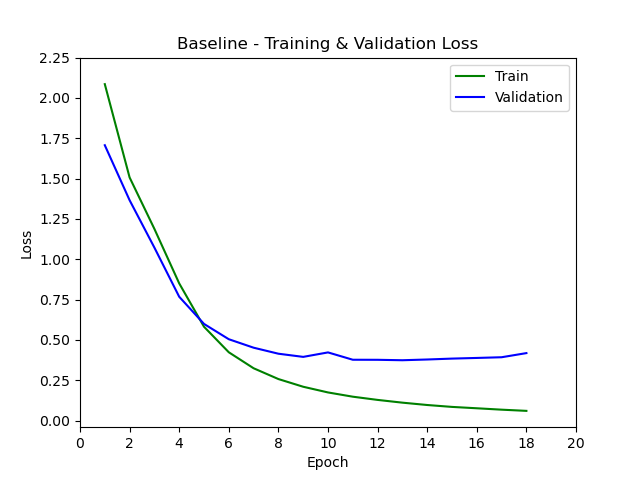
\includegraphics[width=0.6\textwidth]{media/experiments/loss/loss_baseline.png}
\captionsetup{justification=centering}
\caption[Baseline Model Training \& Validation Loss]{Baseline Model Training \& Validation Loss}
\label{fig:loss_baseline}
\end{figure}

%The training set is the only data that will be used to train the model and the validation set is used purely for evaluations during each epoch, identifying whether the model is overfitting and training should be stopped.

%\begin{enumerate}
    %\item 145k sentences
    %\item 5k vocab limit for source and target language
    %\item Mix of original Gaelic and back-translated Gaelic
    %\item Can't do a baseline without the back-translated because the model performs too poorly (basically 0 BLEU score)
    %\item Trained for 20 epochs
%\end{enumerate}




\subsection{Trivial Transfer Learning}
\label{sec:4-trivial}

The trivial transfer learning method that is described in Section \ref{sec:2-transfer_learning} has been implemented using 170,000 sentences from the French dataset as the parent language and 145,000 sentences from the Gaelic dataset as the child language. The parent language was trained for 5 epochs, initialising the child language that was trained for a further 15 epochs. The training and validation loss is shown in Figure \ref{fig:loss_trivial}.



\begin{figure}[ht!]
\centering
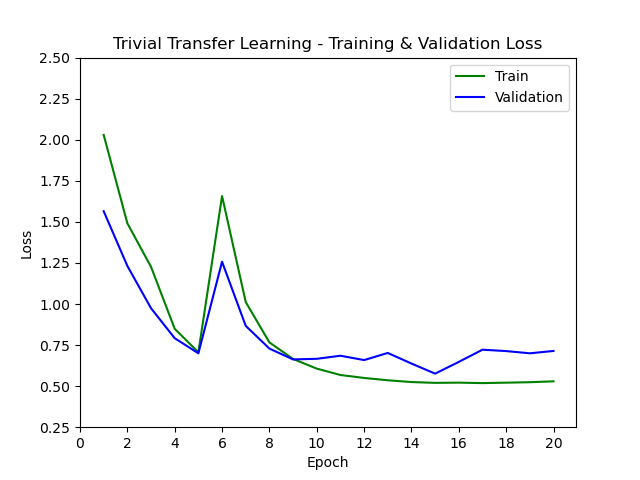
\includegraphics[width=0.6\textwidth]{media/experiments/loss/loss_trivial.png}
\captionsetup{justification=centering}
\caption[Baseline Model Training \& Validation Loss]{Trivial Transfer Learning Model Training \& Validation Loss}
\label{fig:loss_trivial}
\end{figure}



\subsection{Hierarchical Transfer Learning}
\label{sec:4-hierarchical}

The hierarchical transfer learning approach described in Section \ref{sec:2-transfer_learning} has been implemented using French as the parent language, Irish Gaelic as the intermediary language and Scottish Gaelic as the child language.

\begin{enumerate}
    \item Parent dataset: French - 170k sentences, 7k vocab
    \item Intermediary dataset: Irish - 170k sentences, 7k vocab
    \item Child dataset: Gaelic + back-translated Gaelic - 145k sentences, 7k vocab
    \item Trained on parent for 5 epochs
    \item Trained on intermediary for 5 epochs
    \item Trained on child for 15 epochs
\end{enumerate}

\begin{figure}[ht!]
\centering
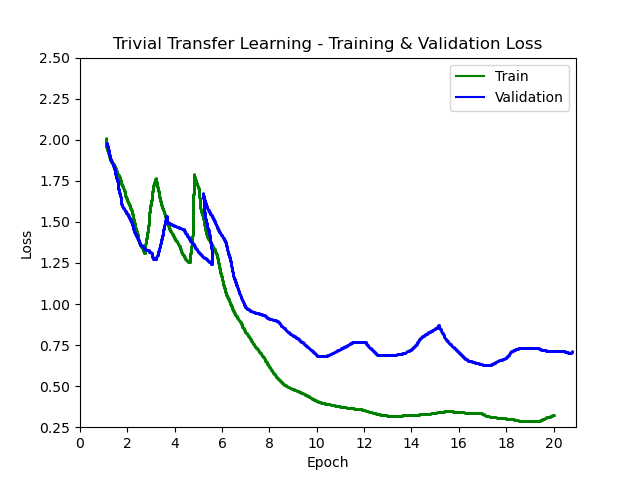
\includegraphics[width=0.6\textwidth]{media/experiments/loss/loss_hierarchical.png}
\captionsetup{justification=centering}
\caption[Baseline Model Training \& Validation Loss]{Hierarchical Transfer Learning Model Training \& Validation Loss \\ \textbf{(SIMULATED RESULTS - TO BE REPLACED)}}
\label{fig:loss_hierarchical}
\end{figure}

\section{Results}

\subsubsection{Vocabulary Size}
As shown in Figure \ref{fig:bleu_vocab}, as vocabulary size increases, so does the translation \acrshort{BLEU} score.

\begin{figure}[ht!]
\centering
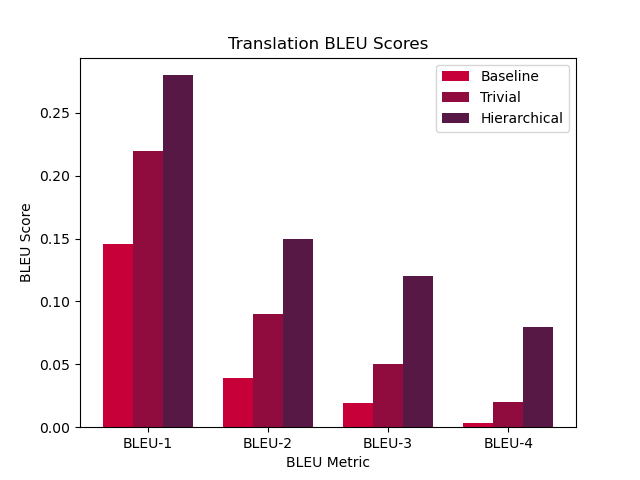
\includegraphics[width=0.85\textwidth]{media/experiments/results/bleu_scores.png}
\captionsetup{justification=centering}
\caption[Baseline Model Training \& Validation Loss]{Baseline Model Training \& Validation Loss}
\label{fig:bleu_vocab}
\end{figure}


\begin{figure}[ht!]
\centering
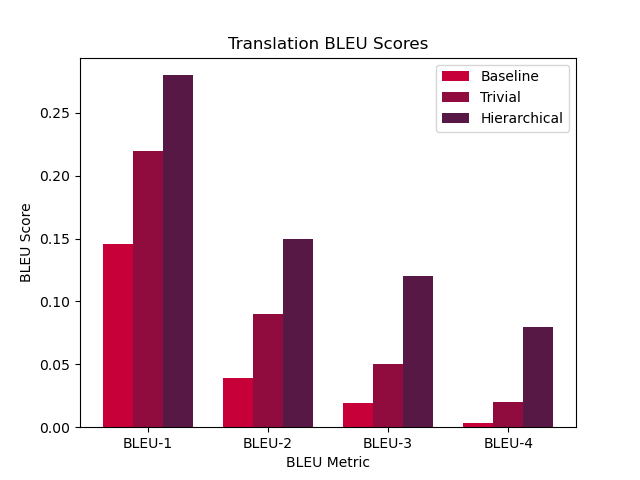
\includegraphics[width=0.85\textwidth]{media/experiments/results/bleu_scores.png}
\captionsetup{justification=centering}
\caption[Experiment BLEU Scores]{Experiment BLEU Scores \textbf{(TEMP FILE - NOT ACTUAL RESULTS)}}
\label{fig:bleu_results}
\end{figure}


Results 1:
\begin{enumerate}
    \item 1-BLEU: X, 2-BLEU: X, 3-BLEU: X, 4-BLEU: X
    \item Attention plot
\end{enumerate}

Results 2:
\begin{enumerate}
    \item 1-BLEU: X, 2-BLEU: X, 3-BLEU: X, 4-BLEU: X
    \item Attention plot
\end{enumerate}

Results 3:
\begin{enumerate}
    \item 1-BLEU: X, 2-BLEU: X, 3-BLEU: X, 4-BLEU: X
    \item Attention plot
\end{enumerate}


\begin{table}[!ht]
\centering
\setlength\doublerulesep{2pt}
\renewcommand{\arraystretch}{1.1}
%\begin{tabular}{|l|p{8cm}|}
\begin{tabular}{|l|l|}
\hline
\multicolumn{2}{|l|}{\textbf{Gaelic \textrightarrow \space English Translation}} \\ \hline
Source          & This is a placeholder sentence.   \\ \hline
Reference       & This is a placeholder sentence.   \\ \hline
Baseline        & This is a placeholder sentence.   \\ \hline
Trivial         & This is a placeholder sentence.   \\ \hline
Hierarchical    & This is a placeholder sentence.   \\ \hhline{==}
Source          & This is a placeholder sentence.   \\ \hline
Reference       & This is a placeholder sentence.   \\ \hline
Baseline        & This is a placeholder sentence.   \\ \hline
Trivial         & This is a placeholder sentence.   \\ \hline
Hierarchical    & This is a placeholder sentence.   \\ \hline
\end{tabular}
\captionsetup{justification=centering}
\caption{Translation sentence analysis}
\label{tab:sentence_analysis}
\end{table}